\documentclass[10pt]{beamer}\usepackage[]{graphicx}\usepackage[]{color}
%% maxwidth is the original width if it is less than linewidth
%% otherwise use linewidth (to make sure the graphics do not exceed the margin)
\makeatletter
\def\maxwidth{ %
  \ifdim\Gin@nat@width>\linewidth
    \linewidth
  \else
    \Gin@nat@width
  \fi
}
\makeatother

\definecolor{fgcolor}{rgb}{0.345, 0.345, 0.345}
\newcommand{\hlnum}[1]{\textcolor[rgb]{0.686,0.059,0.569}{#1}}%
\newcommand{\hlstr}[1]{\textcolor[rgb]{0.192,0.494,0.8}{#1}}%
\newcommand{\hlcom}[1]{\textcolor[rgb]{0.678,0.584,0.686}{\textit{#1}}}%
\newcommand{\hlopt}[1]{\textcolor[rgb]{0,0,0}{#1}}%
\newcommand{\hlstd}[1]{\textcolor[rgb]{0.345,0.345,0.345}{#1}}%
\newcommand{\hlkwa}[1]{\textcolor[rgb]{0.161,0.373,0.58}{\textbf{#1}}}%
\newcommand{\hlkwb}[1]{\textcolor[rgb]{0.69,0.353,0.396}{#1}}%
\newcommand{\hlkwc}[1]{\textcolor[rgb]{0.333,0.667,0.333}{#1}}%
\newcommand{\hlkwd}[1]{\textcolor[rgb]{0.737,0.353,0.396}{\textbf{#1}}}%
\let\hlipl\hlkwb

\usepackage{framed}
\makeatletter
\newenvironment{kframe}{%
 \def\at@end@of@kframe{}%
 \ifinner\ifhmode%
  \def\at@end@of@kframe{\end{minipage}}%
  \begin{minipage}{\columnwidth}%
 \fi\fi%
 \def\FrameCommand##1{\hskip\@totalleftmargin \hskip-\fboxsep
 \colorbox{shadecolor}{##1}\hskip-\fboxsep
     % There is no \\@totalrightmargin, so:
     \hskip-\linewidth \hskip-\@totalleftmargin \hskip\columnwidth}%
 \MakeFramed {\advance\hsize-\width
   \@totalleftmargin\z@ \linewidth\hsize
   \@setminipage}}%
 {\par\unskip\endMakeFramed%
 \at@end@of@kframe}
\makeatother

\definecolor{shadecolor}{rgb}{.97, .97, .97}
\definecolor{messagecolor}{rgb}{0, 0, 0}
\definecolor{warningcolor}{rgb}{1, 0, 1}
\definecolor{errorcolor}{rgb}{1, 0, 0}
\newenvironment{knitrout}{}{} % an empty environment to be redefined in TeX

\usepackage{alltt}
\usetheme{metropolis}           % Use metropolis theme

\usepackage{graphicx}

\DeclareGraphicsExtensions{.pdf,.jpeg,.jpg,.png}

\usepackage{subcaption}
\usepackage{amsmath}

\usepackage{tikz}
\usetikzlibrary{bayesnet}
\usepackage{pgfplots}
\pgfplotsset{compat=1.13}

\usepackage[framemethod=TikZ, xcolor=RGB]{mdframed}
\definecolor{mydarkblue}{rgb}{0,.06,.5}
\definecolor{mydarkred}{rgb}{.5,0,.1}
\definecolor{myroyalblue}{rgb}{0,.1,.8}
\mdfdefinestyle{MyFrame}{%
    linecolor=mydarkblue,
    outerlinewidth=0.5pt,
    roundcorner=2pt,
    innertopmargin=2pt,
    innerbottommargin=2pt,
    innerrightmargin=2pt,
    innerleftmargin=2pt,
    backgroundcolor=blue!10}

\newcommand{\Rbb}{\mathbb{R}}
\newcommand{\Expect}{\mathbb{E}}
\newcommand{\Expecthat}{\hat{\mathbb{E}}}
\newcommand{\Var}{\text{Var}}
\newcommand{\Cov}{\text{Cov}}

\renewcommand{\t}{t}

\DeclareMathOperator*{\argmin}{arg\,min}





\title{Evaluating Sensitivity to the Stick Breaking Prior in
Bayesian Nonparametrics}
\date{April 26, 2021}
\author{Runjing (Bryan) Liu}
\institute{University of California, Berkeley}

\setbeamertemplate{Collaborators}[none]
\IfFileExists{upquote.sty}{\usepackage{upquote}}{}
\begin{document}
\maketitle

\begin{frame}{Collaborators}
  	\vspace{1em}
  	\begin{figure}
  		\begin{subfigure}{.4\textwidth}
  			\centering
  			
\includegraphics[height=2cm]{collaborators/bryan}
        \captionsetup{justification=centering}
  			\caption*{Runjing (Bryan) Liu \\ UC Berkeley}
  		\end{subfigure}%
  		\begin{subfigure}{.4\textwidth}
  			\centering
  			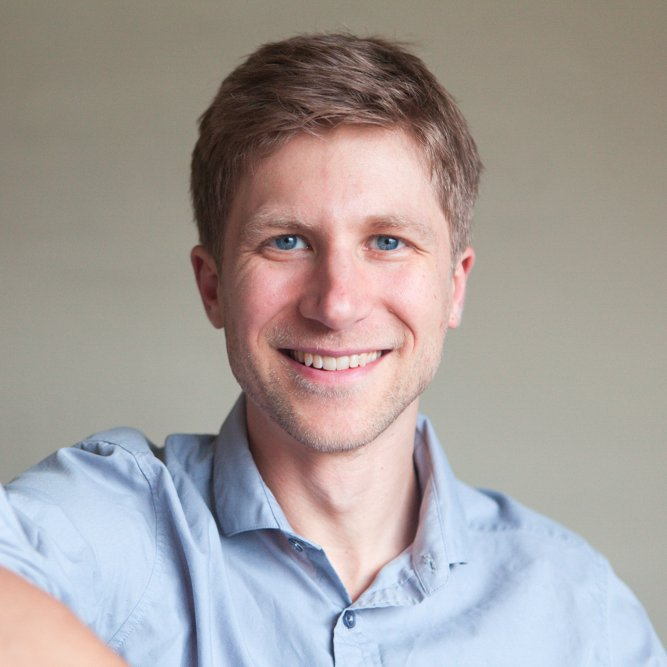
\includegraphics[height=2cm]{collaborators/ryan}
  			\caption*{Ryan Giordano \\ MIT}
  		\end{subfigure}\\ \vspace{0.11in}
      \begin{subfigure}{.4\textwidth}
  			\centering
  			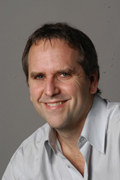
\includegraphics[height=2cm]{collaborators/mike}
  			\caption*{Michael I.\ Jordan \\ UC Berkeley}
  		\end{subfigure}%
  		\begin{subfigure}{.4\textwidth}
  			\centering
  			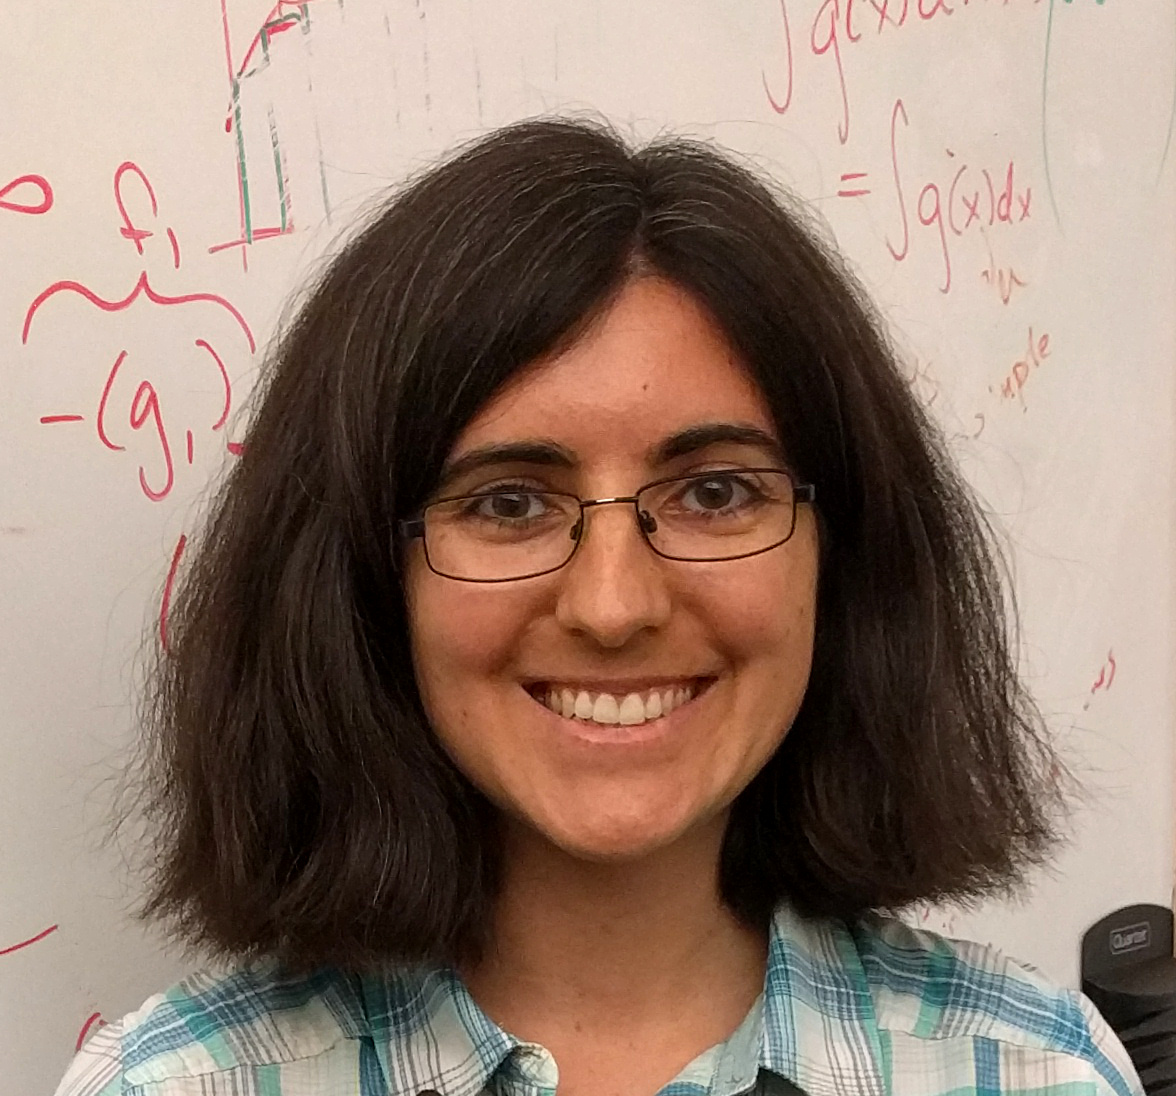
\includegraphics[height=2cm]{collaborators/tamara}
  			\caption*{Tamara Broderick \\ MIT}
  		\end{subfigure}\\
  	\end{figure}

\end{frame}


\begin{frame}{Motivation}

Inferring population structure from genomic sequences.
\begin{itemize}
  \item[--] Genetic data from Taita thrush, an endagered bird species native to Kenya
  {\color{blue} \href{https://web.stanford.edu/group/pritchardlab/publications/pdfs/PritchardEtAl00.pdf}{(Pritchard et al. 2011)}}.

  \item[--] Microsatellites sequences of 155 individiuals at 7 loci.
\end{itemize}


\begin{figure}[!h]
\centering
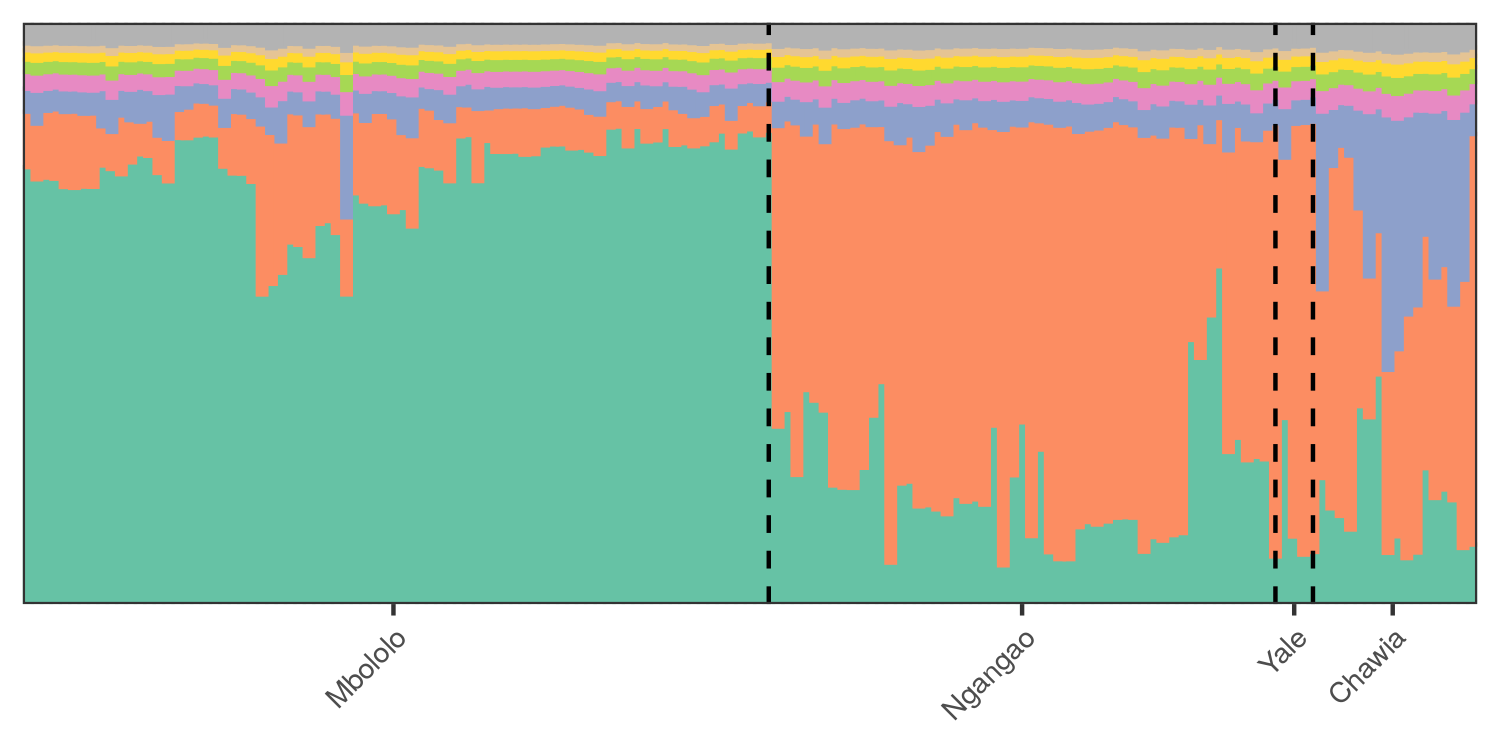
\includegraphics[width = 0.8\textwidth]{./figures/structure_example.png}
\end{figure}

\end{frame}

\begin{frame}{Motivation}

\begin{figure}[!h]
\centering
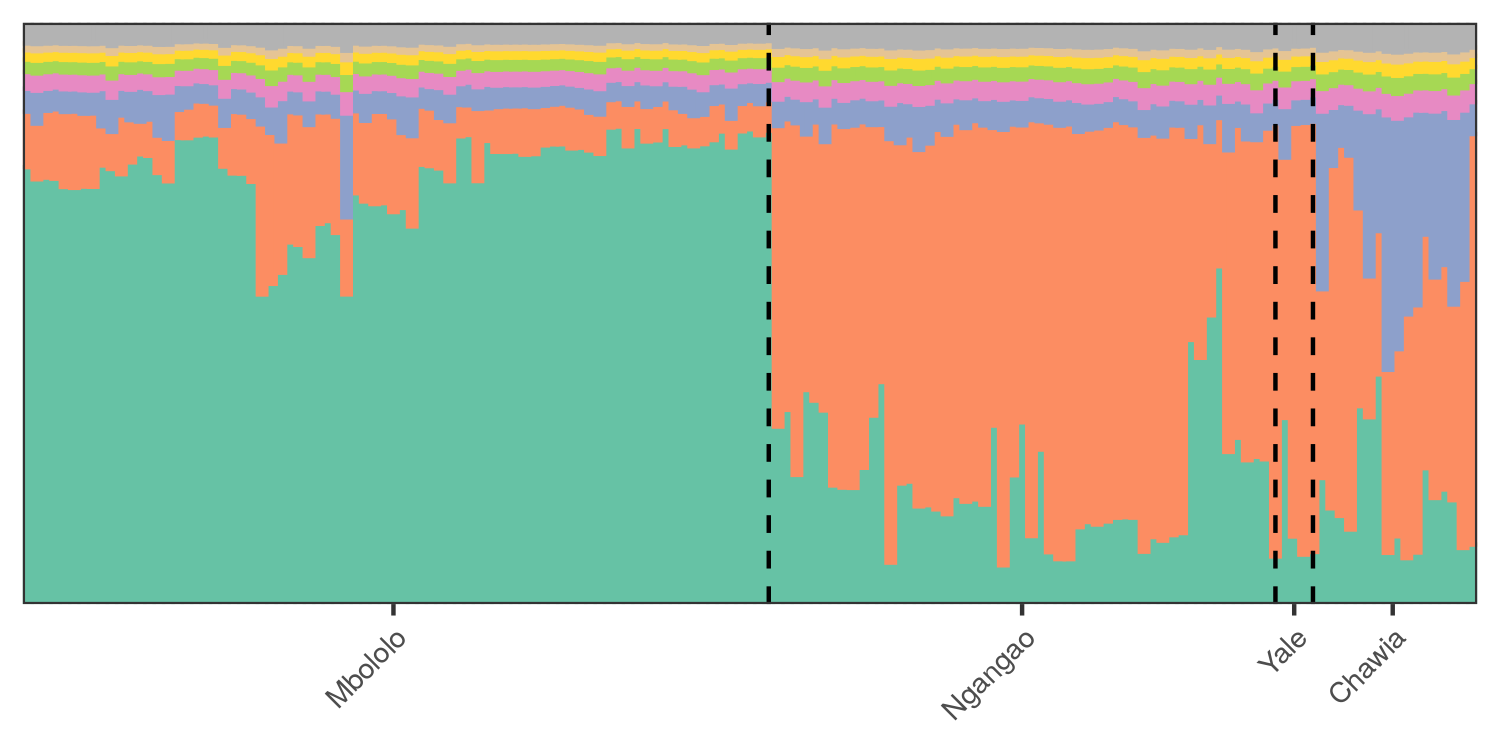
\includegraphics[width = 0.8\textwidth]{./figures/structure_example.png}
\end{figure}

\vspace{-1em}

{\bf Possible questions of interest: }

\begin{enumerate}
    \item How many latent populations---aka clusters---are present in the data set?
    \pause
    \item Which individuals cluster together?
    \pause
    \item What are the unique characterstics of each cluster?
\end{enumerate}


\end{frame}
\begin{frame}{Research problem}

A Bayesian nonparametric (BNP) model makes inferring the number of clusters amenable to
Bayesian inference.

\pause

We approximate the exact posterior using variational Bayes.

\pause

\textbf{Question}: how sensitive is the VB approximation, and the resulting
inferences, to BNP model choices?

\pause

\textbf{Problem}: re-running VB for multiple model choices is expensive.

\pause

\textbf{We propose}: a linear approximation to efficiently
estimate BNP sensitivity from a single run of VB (to avoid
expensive refitting).

\end{frame}

\begin{frame}{Outline}
\begin{itemize}
\item The BNP model
\vspace{0.1in}

\item The variational approximation
\vspace{0.1in}

\item Hyperparameter sensitivity
\vspace{0.1in}

\item Functional sensitivity and influence functions
\vspace{0.1in}

\item Results on population genetics modeling of the Taita thrush 
\vspace{0.1in}

\end{itemize}
\end{frame}


\begin{frame}{The BNP Model}
A {\bf Dirichlet process prior} allows for an infinite number of components.
\vspace{-0.2in}
\begin{figure}[!h]
\centering
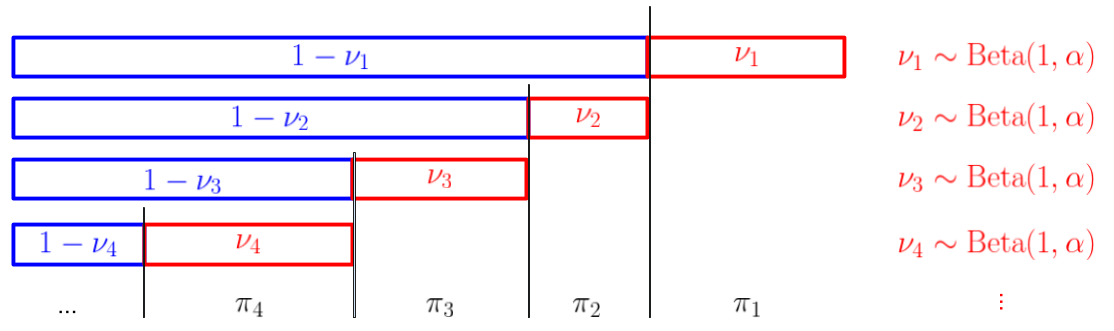
\includegraphics[width = 0.95\textwidth]{./figures/static_figures/DP_stick_breaking.png}
\caption{A schematic of the Dirichlet process prior}
\end{figure}
\vspace{-0.2in}

While there are an infinite number of {\bf components}, there are a finite number of {\bf clusters} in a given dataset. \pause We might ask:

\begin{enumerate}[(1)]
\item How many clusters are in the {\itshape current} dataset?

\pause
\item Given our current knowledge, how many clusters would we expect to see in a {\itshape new} dataset?

\end{enumerate}

\pause

These quantities depend on the choice of stick-breaking prior.

\pause

\begin{mdframed}[style=MyFrame]
\begin{center}
{\bf What makes this stick-breaking prior a reasonable one?}
\end{center}
\end{mdframed}

\end{frame}


\begin{frame}{The Variational Approximation}

Let $\theta$ be latent variables and $y$ the observed data.
The exact posterior $p(\theta | y)$ is intractable.

We posit a class of distributions $\mathcal{Q}$ parameterized by a real vector $\eta$.
We solve
\begin{align*}
  \eta^* = \argmin_{\eta} KL\left(
      q(\theta \vert \eta )\big\| p(\theta | y)
      \right)
\end{align*}

\only<1>{
\vspace{-1em}
\begin{figure}[!h]
\centering
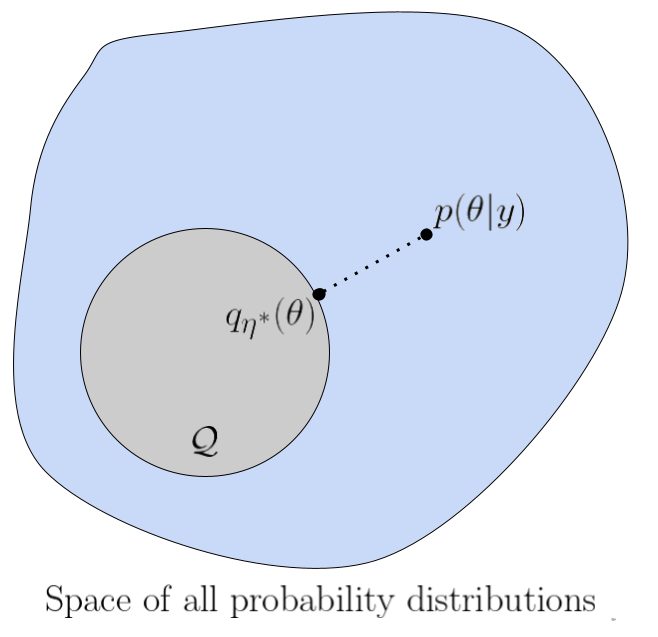
\includegraphics[width = 0.4\textwidth]{./figures/static_figures/vi_schematic2.png}
\end{figure}
}

\only<2->{
Note that

\begin{itemize}
\item The optimal variational parameters $\eta^*$ depend on the prior through optimizing the KL objective.

\pause

\item The approximate posterior quantities are then functions of $\eta^*$, e.g.\
\begin{align*}
\eta^* \mapsto
\Expect_{q_{\eta^*}} \left[ \#\text{clusters} \right]
\quad \text{ or } \quad
\eta^* \mapsto
\Expect_{q_{\eta^*}}
\left[\#\{\substack{\text{clusters in}\\\text{new dataset}}\} \right].
\end{align*}

\end{itemize}
}

\only<3>{
\begin{mdframed}[style=MyFrame]
\begin{center}
{\bf How do these approximate posterior quantities depend on the DP prior?}
\end{center}
\end{mdframed}
}
\end{frame}


\begin{frame}{Hyperparameter Sensitivity}

Let $\t$ be a real-valued hyperparameter for the stick-breaking distribution
(e.\ g., this could be the $\alpha$ concentration parameter, or it could parameterize a functional shape).

\pause

{\bf Main idea: } We approximate the dependence of $\eta^*$ on $\t$ with a first-order
Taylor expansion:

\begin{align*}
  \eta^*(\t)  &\approx  \eta^*(0) +
  \frac{d \eta^*(\t)}{d\t}\Big|_{\t=0} \t
\end{align*}

\pause

Notes:
\begin{itemize}
\item Evaluation of the derivative can be done efficiently using formulas from
{\color{blue} \href{https://arxiv.org/abs/1709.02536}{Giordano et al. 2018}}
and modern
{\color{blue} \href{https://jax.readthedocs.io/en/latest/}{automatic differentiation tools}}.

\item We only use a linear approximation for the map $\t \mapsto \eta^*(\t)$. We retain nonlinearities in the map $\eta^* \mapsto
\Expect_{q_{\eta^*}} \left[ \#\text{clusters} \right]$.

\end{itemize}
\end{frame}

\begin{frame}{A simple example: iris data}

We fit a Gaussian mixture model with a DP prior to
the iris data.

\begin{figure}[!h]
  \centering
  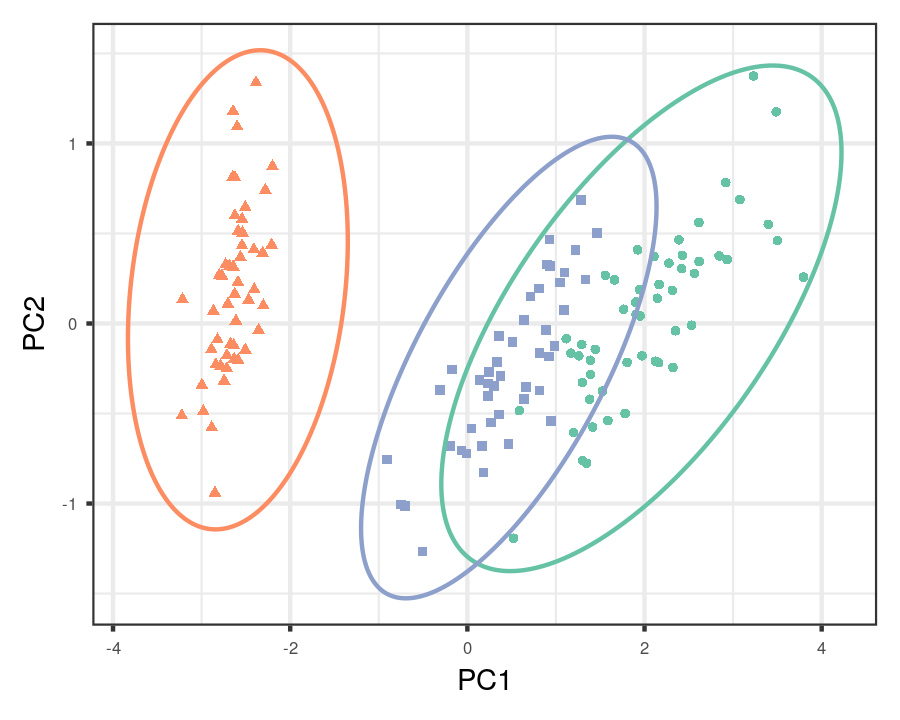
\includegraphics[width = 0.6\textwidth]{./figures/iris_init_fit.png}
  \caption*{The iris data in principal component space and GMM fit at $\alpha = 6$.}
\end{figure}

\end{frame}

\begin{frame}{iris data: parametric sensitivity}

\begin{figure}[!h]
  \only<1>{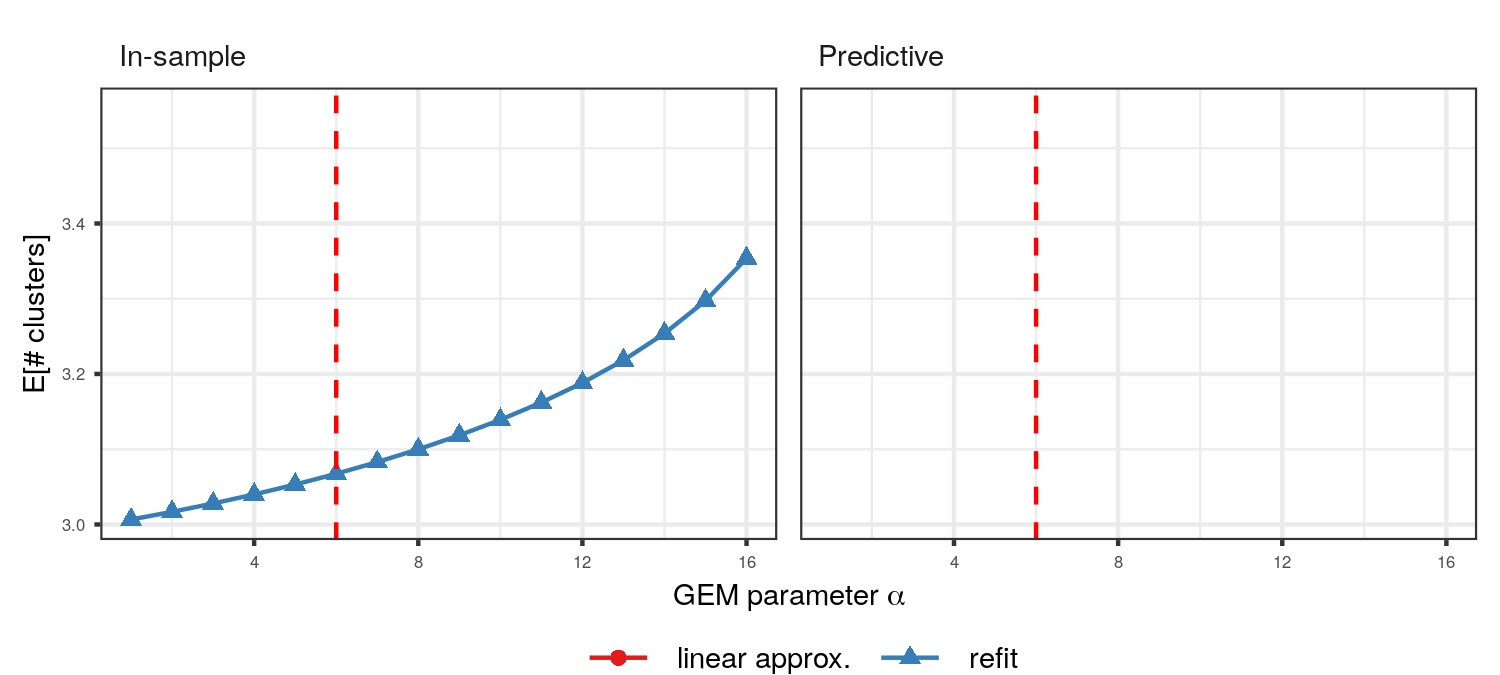
\includegraphics[width = \textwidth]{./figures/iris_alpha_sens0.png}}%
  \only<2>{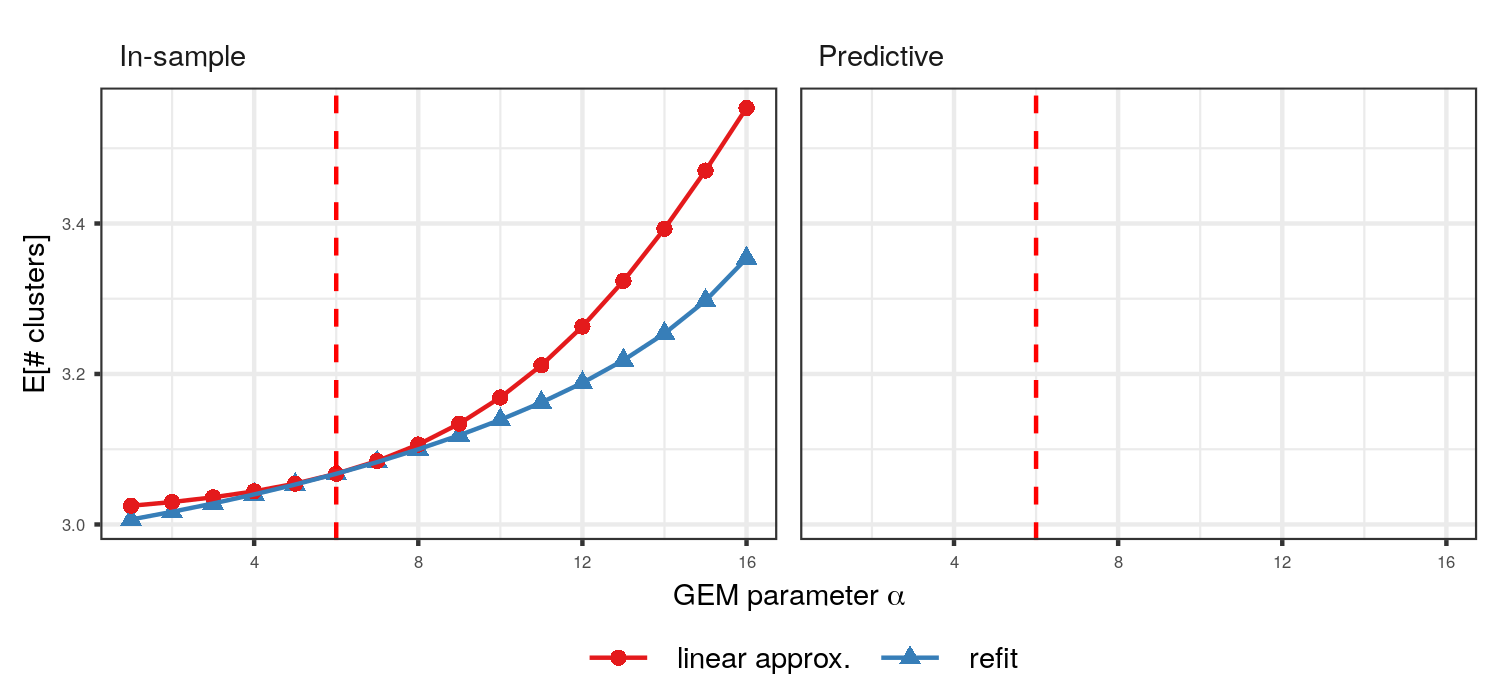
\includegraphics[width = \textwidth]{./figures/iris_alpha_sens1.png}}%
  \only<3>{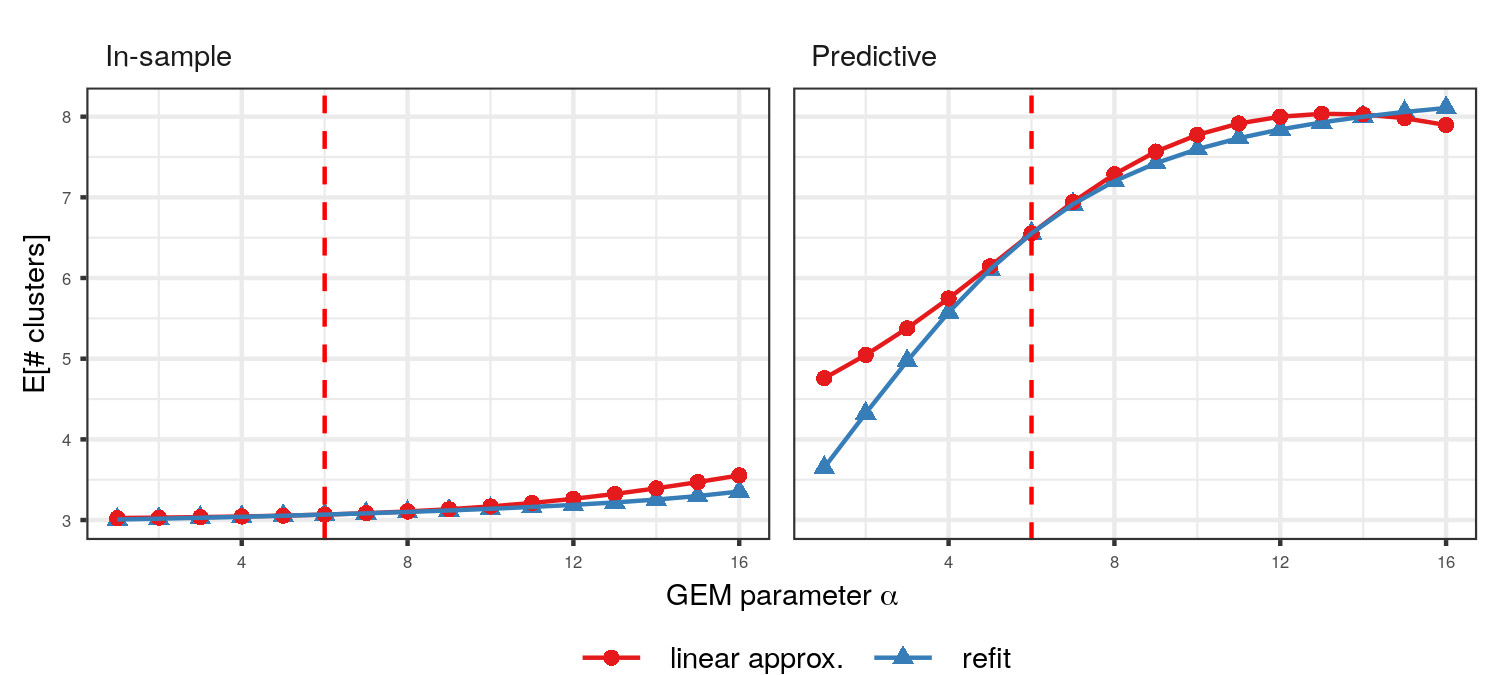
\includegraphics[width = \textwidth]{./figures/iris_alpha_sens2.png}}
  \caption*{The expected number of posterior clusters in the iris data as $\alpha$ varies.}
\end{figure}

\end{frame}


\begin{frame}{Functional sensitivity}
Let $p_0(\nu_k)$ be the original Beta prior on sticks.

Suppose we wish to replace $p_0$ with another distribution $p_1$. Define the ``contaminated" prior as:
\begin{align*}
p_c(\nu_k \vert \epsilon) \propto
p_{0}(\nu_k)\exp(\epsilon\phi(\nu_k))
\end{align*}
where $\phi(\nu_k) = \log p_1(\nu_k) - \log p_0(\nu_k)$.

\begin{figure}[!h]
\centering
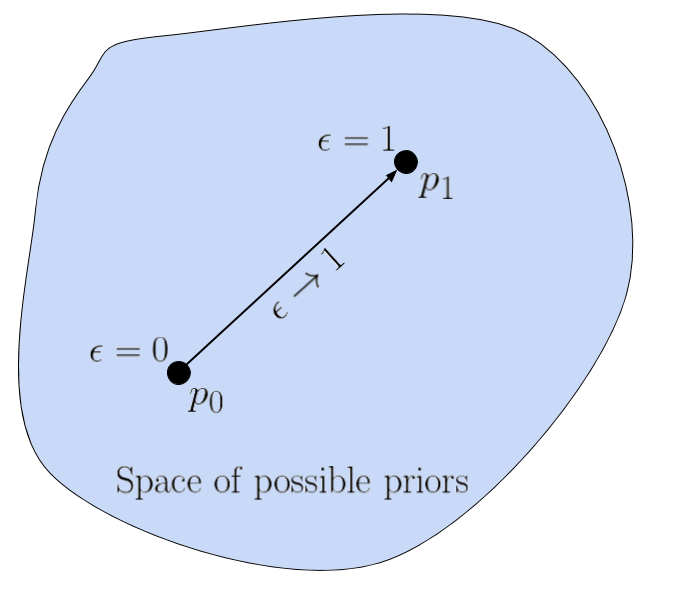
\includegraphics[width = 0.45\textwidth]{./figures/static_figures/functional_perturbation.png}
\setlength{\textfloatsep}{-10pt}
\end{figure}

\end{frame}

\begin{frame}{Functional sensitivity: influence functions}

Consider a posterior statistic of interest $g(\eta)$, e.g.
\begin{align*}
g_{\textrm{cl}}(\eta) = \Expect_{q_{\eta}} \left[ \#\text{clusters} \right]
\end{align*}

Let $S_g$ be the \textit{local sensitivity} of $g$ with respect to a hyper-parameter $\epsilon$
\begin{align*}
S_g := \frac{d}{d\epsilon} \; g(\eta(\epsilon))
\end{align*}

\pause

The local sensitivity can be expressed as an inner-product between an \textit{influence function} $\Psi$
and the functional perturbation $\phi$ in an appropriate Hilbert space:
\begin{align*}
S_g &= \langle \Psi, \phi\rangle \\
&= \int \Psi(\nu) \phi(\nu) p_0(\nu) \;d\nu
\end{align*}


\end{frame}

\begin{frame}{Iris data: influence functions}
  \begin{figure}[!h]
    \centering
    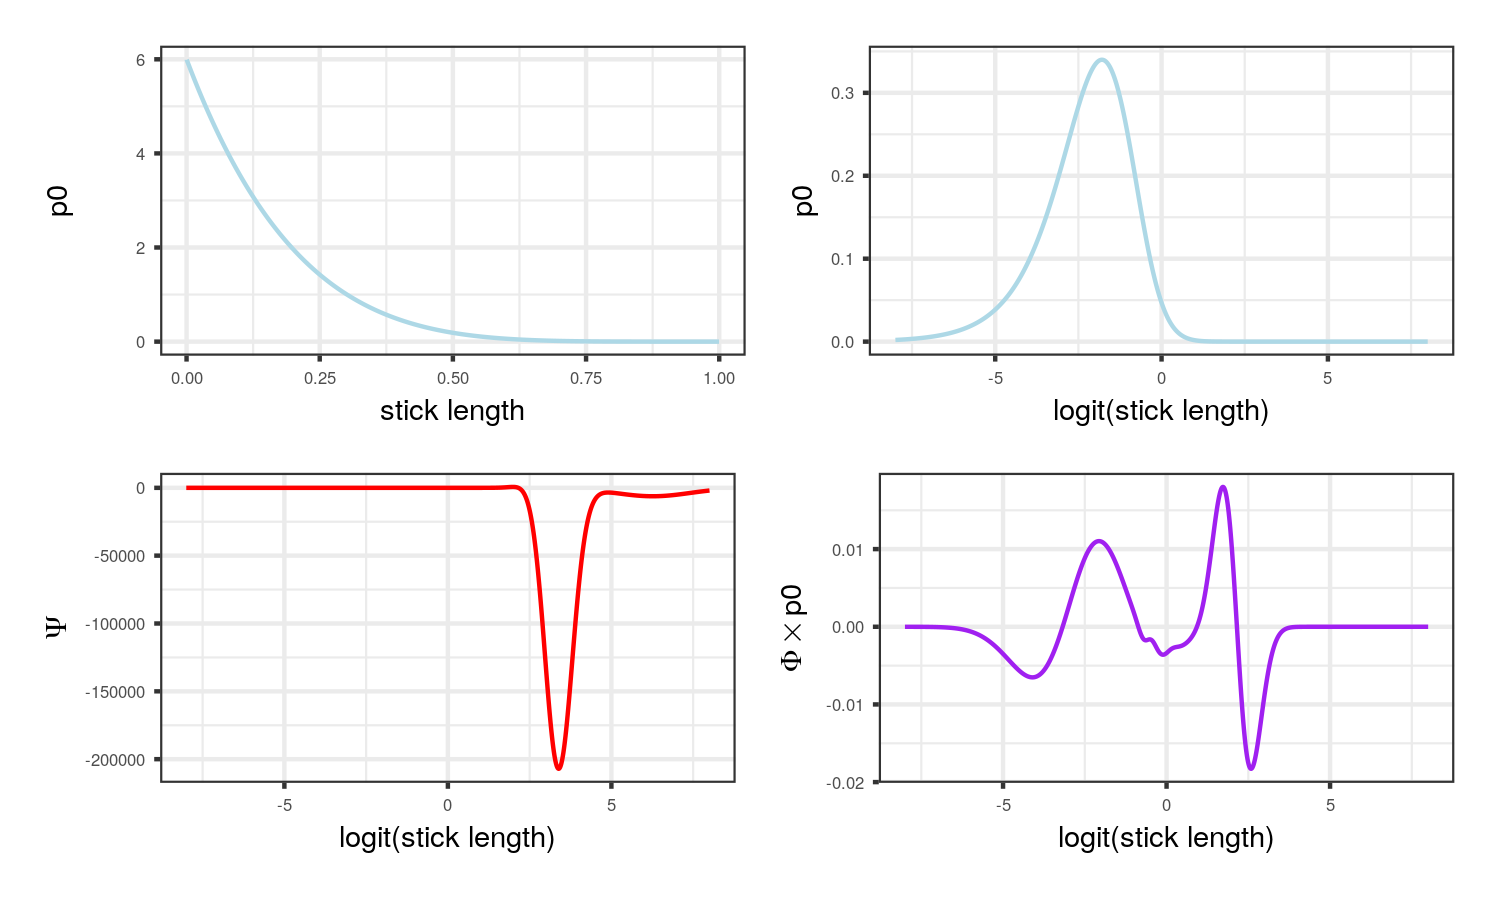
\includegraphics[width = \textwidth]{./figures/iris_influence_function.png}
    \caption*{The influence function for the number of clusters, $g_{\textrm{cl}}$.}
\end{figure}
\end{frame}

\begin{frame}{Iris data: functional perturbations}
\begin{figure}[!h]
    \centering
    \only<1>{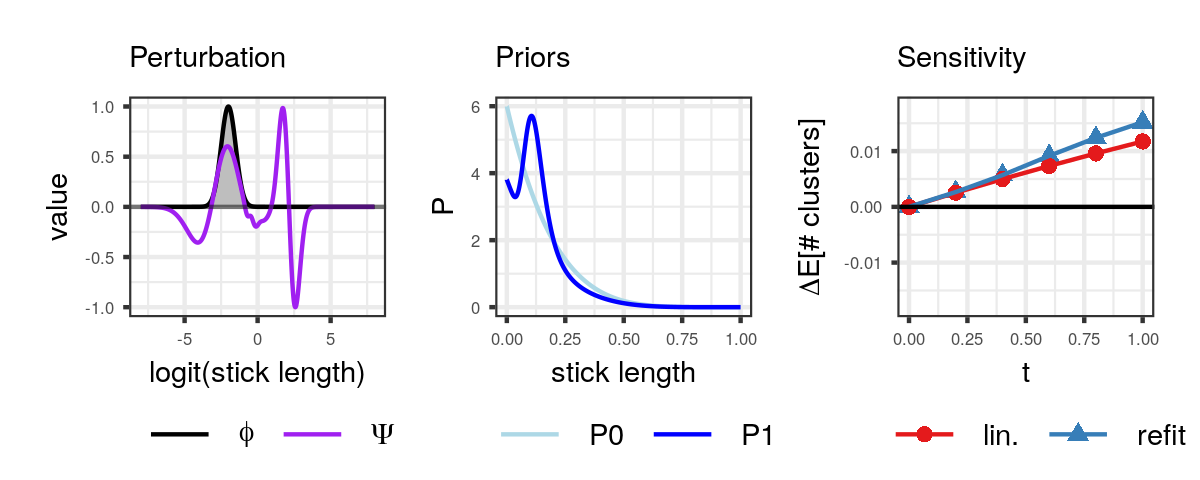
\includegraphics[width = 0.8\textwidth]{./figures/iris_func_sens0.png}}
    \only<2>{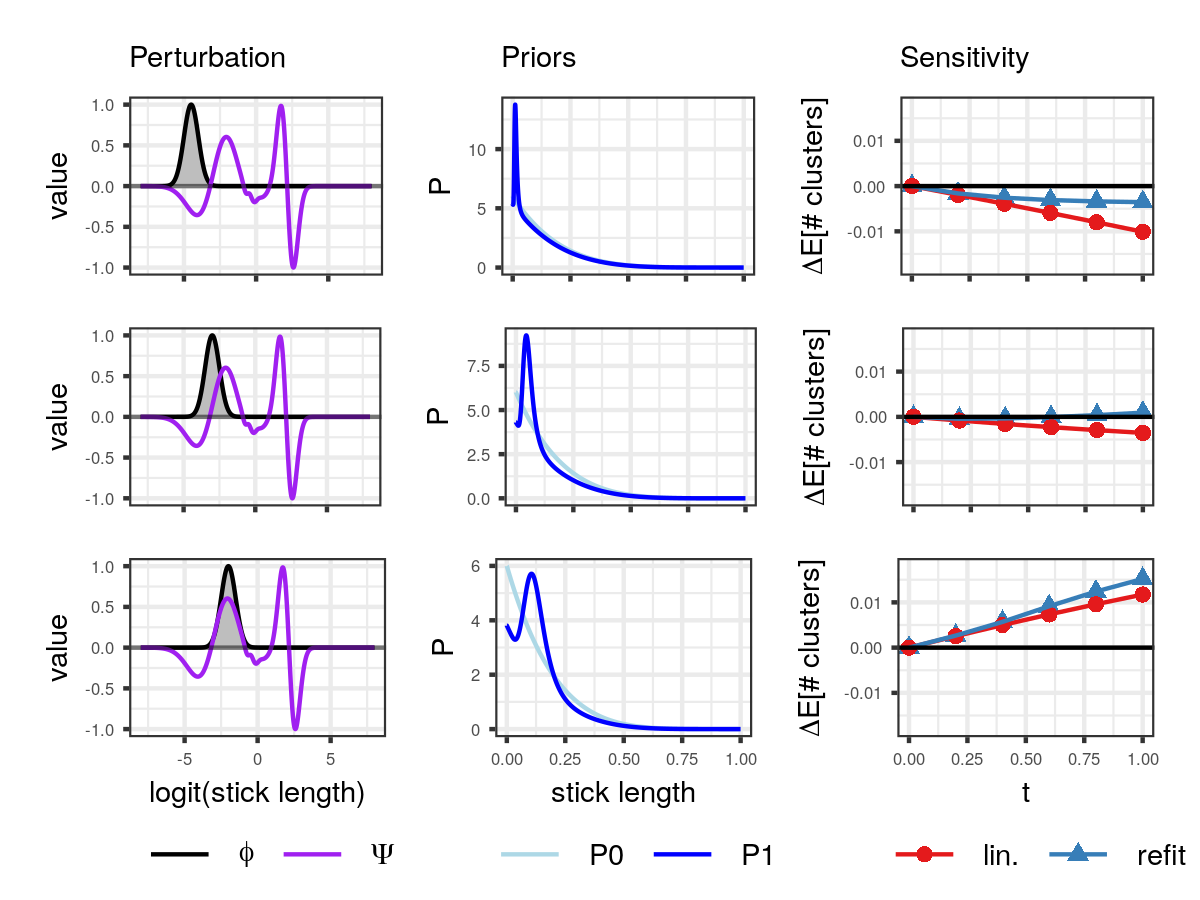
\includegraphics[width = 0.8\textwidth]{./figures/iris_func_sens1.png}}
\end{figure}
\end{frame}

\begin{frame}{Functional perturbations: worst-case}

There are many possible choices for $p_1$.

Given a posterior quantity $g$,
we can find the {\itshape worst-case} perturbation in a ball of
radius $\delta$, that is, find the direction such that
$|S_g|$ is maximized.

\vspace{-1em}

\begin{figure}[!h]
\centering
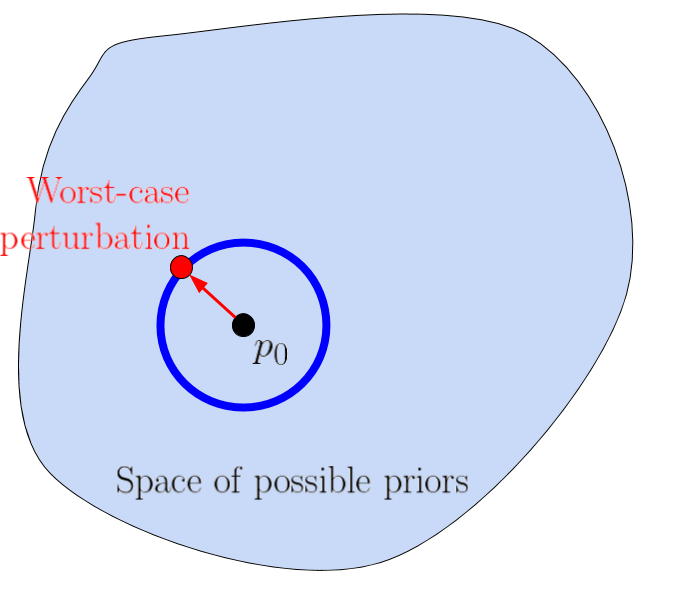
\includegraphics[width = 0.4\textwidth]{./figures/static_figures/functional_perturbation_worst_case.png}
\setlength{\textfloatsep}{-10pt}
\end{figure}

\vspace{-1em}

Specifically, we consider the L-infinity ball of radius $\delta$:
\begin{align*}
  B_\delta := \{\phi : \|\phi\|_\infty < \delta\}
\end{align*}

\end{frame}

\begin{frame}{Iris data: worst-case perturbation}
  \begin{figure}[!h]
    \centering
    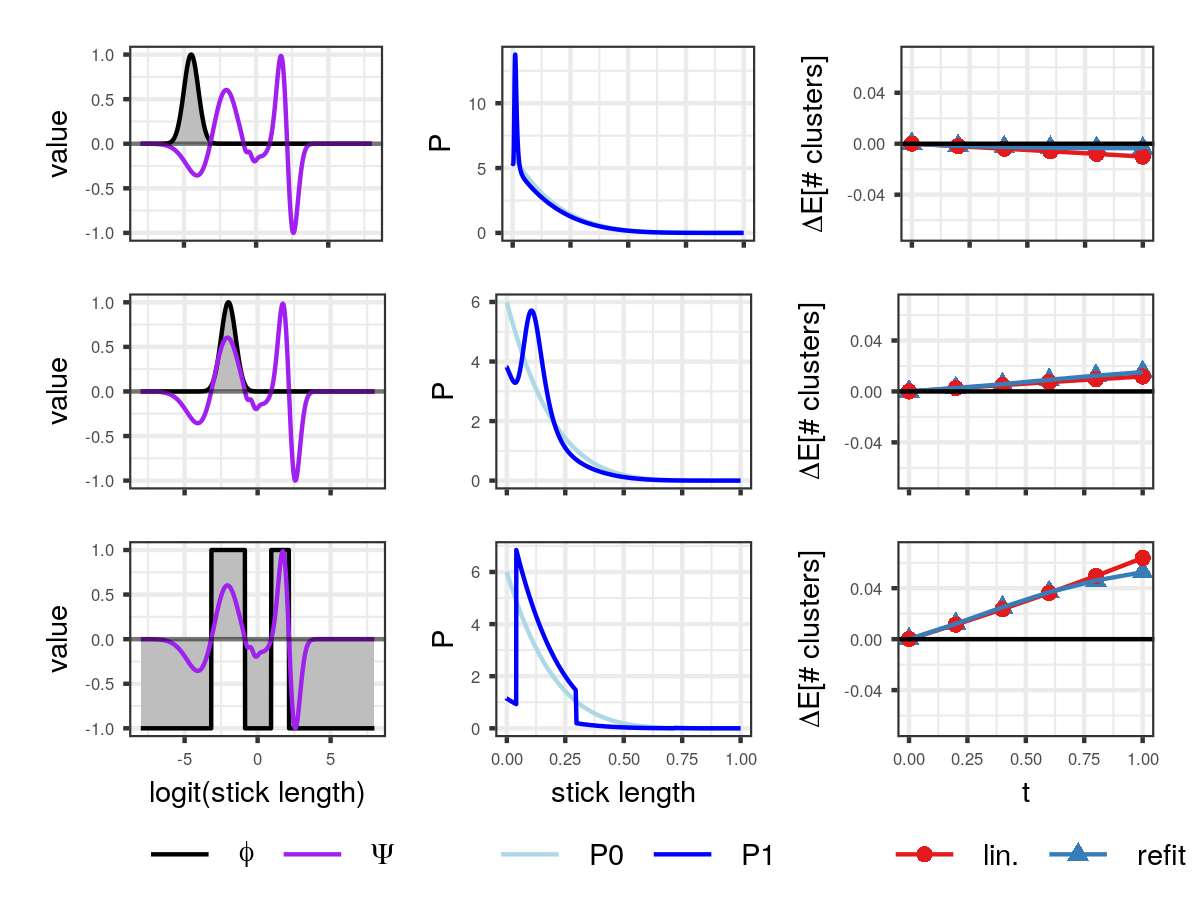
\includegraphics[width = 0.8\textwidth]{./figures/iris_worst_case.png}
\end{figure}
\end{frame}


\begin{frame}{Results on STRUCTURE}

We adapt STRUCTURE
{\color{blue} \href{https://web.stanford.edu/group/pritchardlab/publications/pdfs/PritchardEtAl00.pdf}{(Pritchard et al. 2011};
\href{https://www.genetics.org/content/197/2/573}{Raj et al. 2014)}
},
a Bayesian model for population genetics, to include a BNP prior.


We study genetic data from the Taita thrush, an endagered bird species.
The data consists of microsatellites sequences of 155 individiuals at 7 loci.

\begin{figure}[!h]
\centering
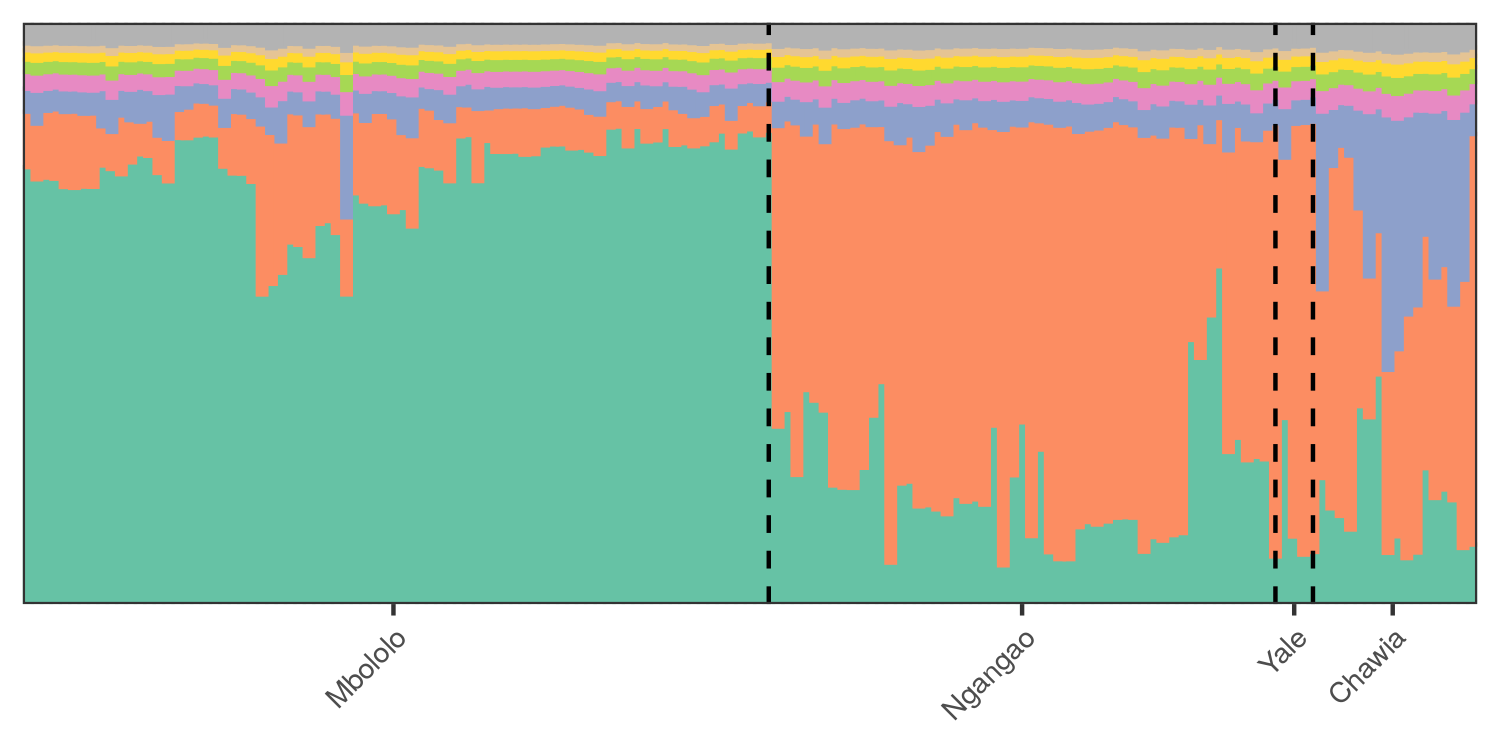
\includegraphics[width = 0.8\textwidth]{./figures/structure_example.png}
\caption{The intitial fit at $\alpha = 3$. }
\end{figure}
\end{frame}

\begin{frame}{STRUCTURE: parametric sensitivity}
  \begin{figure}[!h]
    \centering
    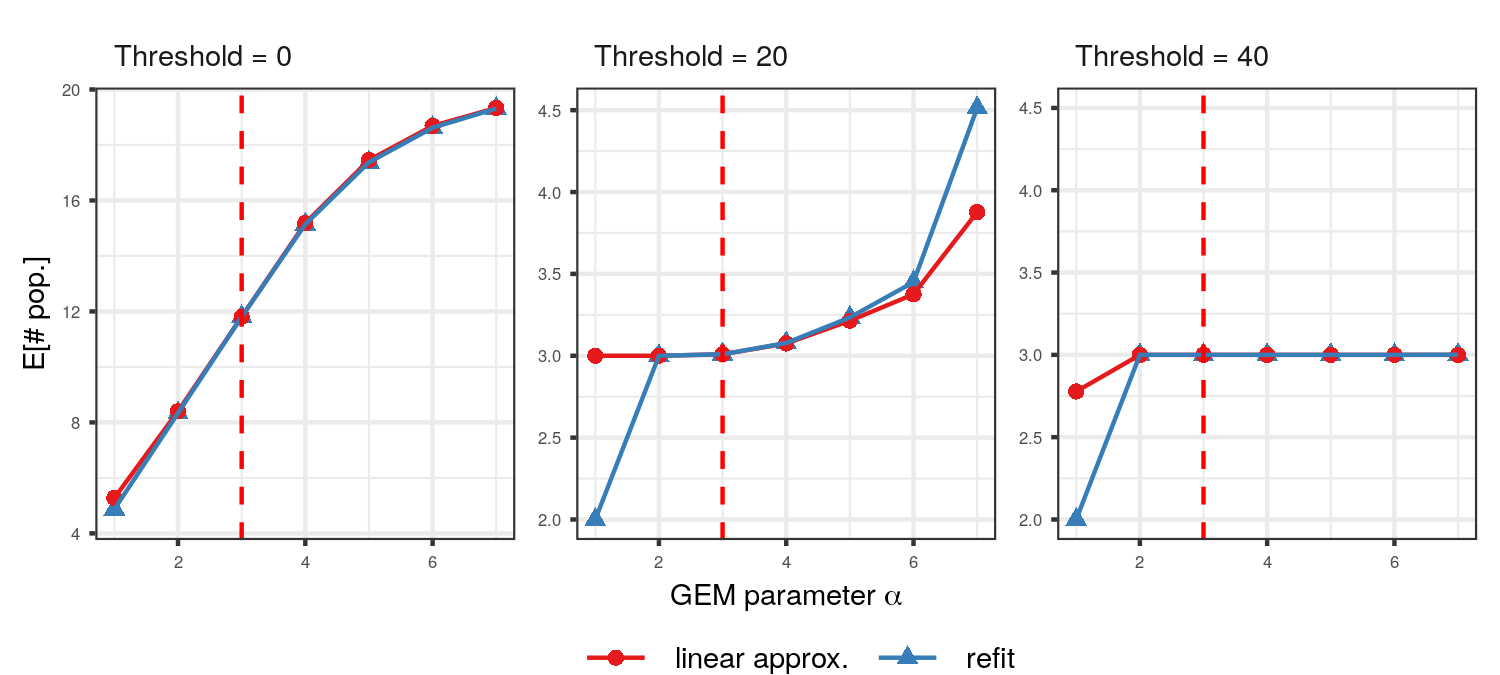
\includegraphics[width = \textwidth]{./figures/stucture_alpha_sens.png}
    \caption*{The expected number of posterior in-sample clusters in the thrush data as $\alpha$ varies.}
  \end{figure}

\end{frame}

\begin{frame}{STRUCTURE: functional sensitivity}

  \begin{figure}[!h]
    \centering
    \only<1>{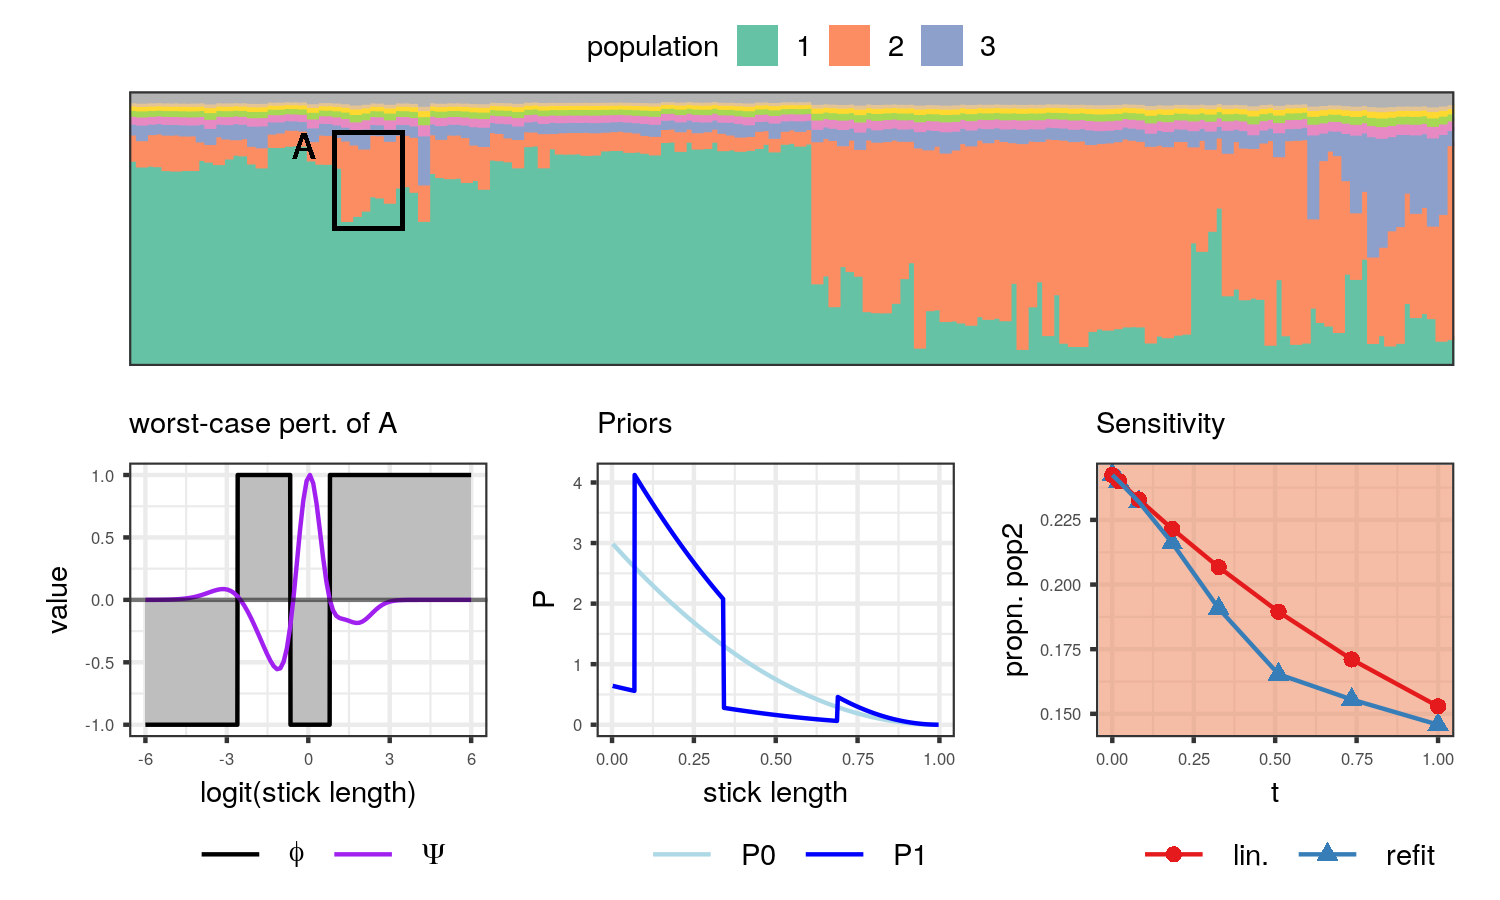
\includegraphics[width = \textwidth]{./figures/structure_mbololo_sens.png}}%
    \only<2>{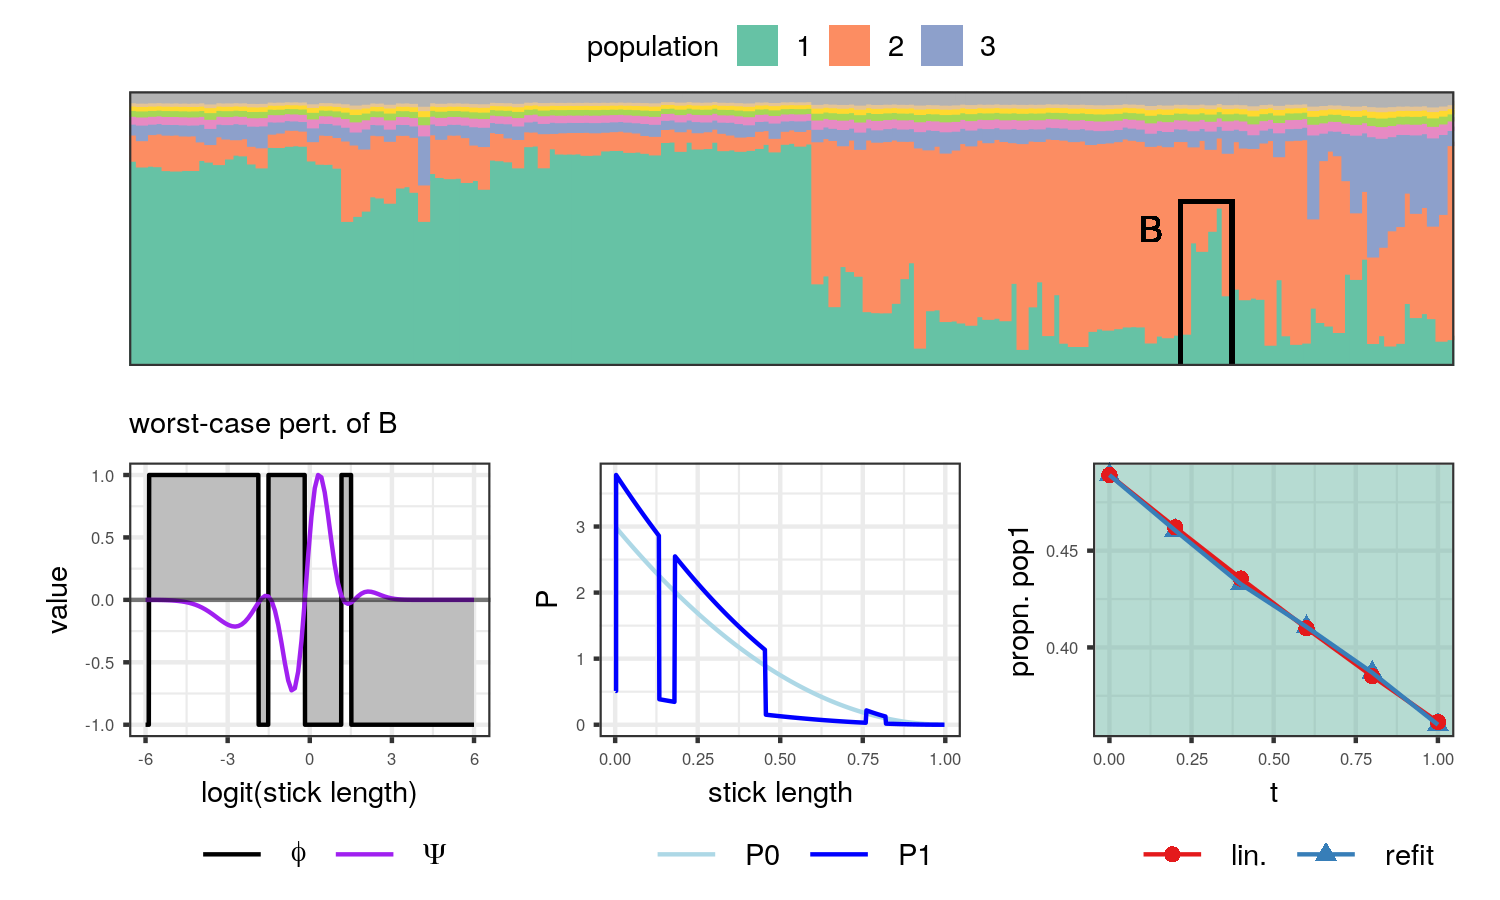
\includegraphics[width = \textwidth]{./figures/structure_ngangao_sens.png}}%
    \only<3>{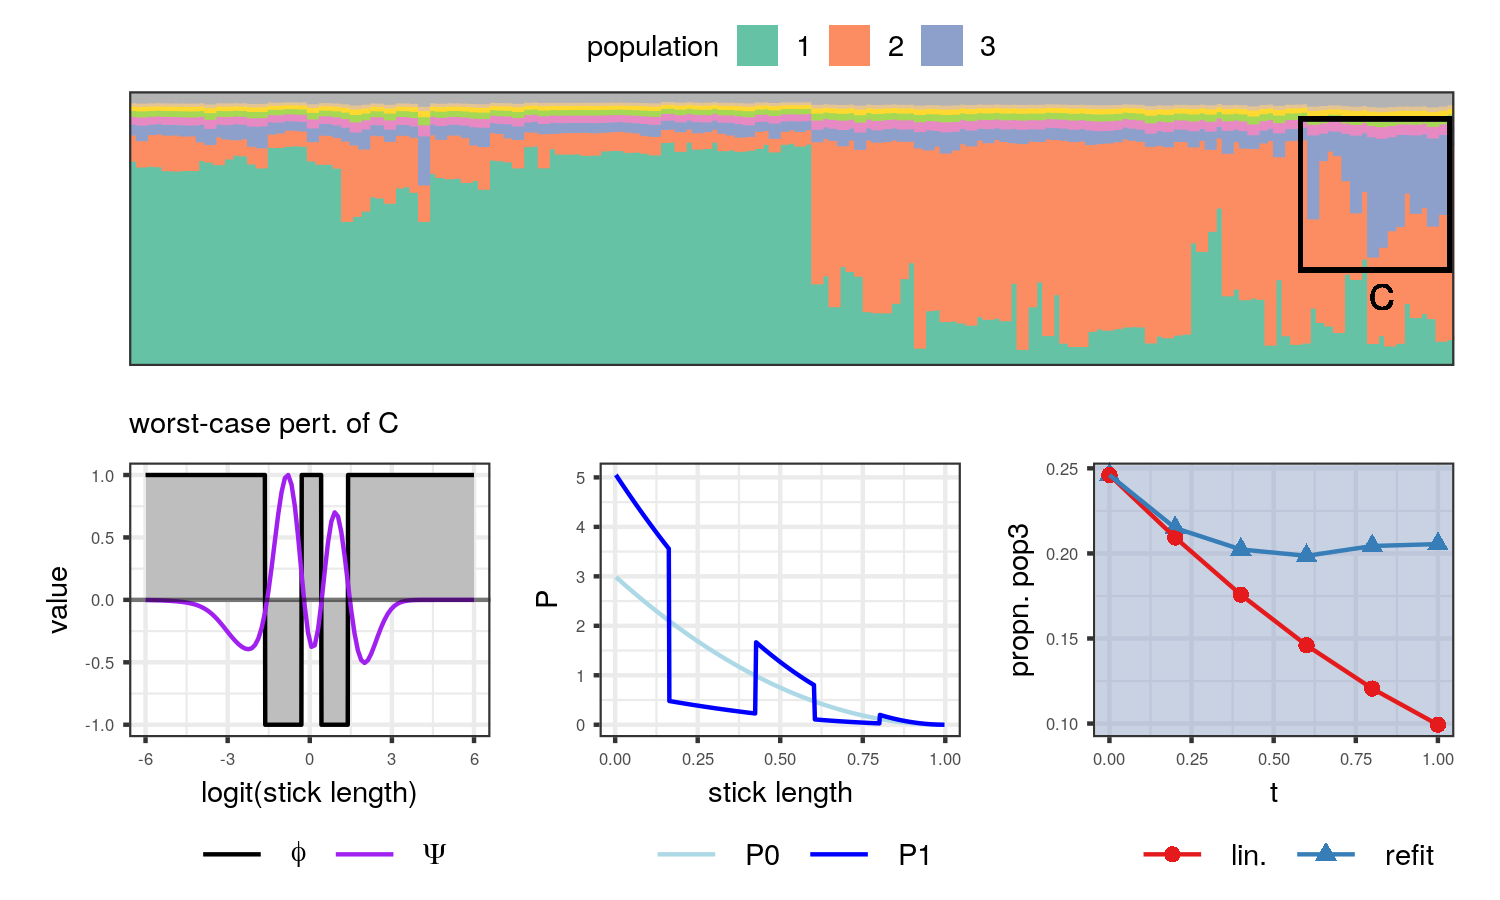
\includegraphics[width = \textwidth]{./figures/structure_chawia_sens.png}}
  \end{figure}

\end{frame}

\begin{frame}{Computational times}

\begin{table}[tb]
\centering
\caption*{Compute time of results on the Taita thrush dataset. }
\begin{tabular}{|r|r|}
\hline
    & time (seconds) \\
    \hline
    Initial fit & 7 \\
    \hline
    Hessian solve for $\alpha$ sensitivity & 0.3\\
    Linear approx. $\eta^{lin}(\alpha)$ for $\alpha = 1, ..., 7$ &
        0.006 \\
    Refits $\eta(\alpha)$ for $\alpha = 1, ..., 7$ &
        30 \\
    \hline
    The influence function & 0.6 \\
    Hessian solve for worst-case $\phi$ &
        0.4 \\
    Linear approx. $\eta^{lin}(\epsilon)|_{\epsilon = 1}$
      for worst-case $\phi$ &
        0.001\\
    Refit $\eta(\epsilon)|_{\epsilon = 1}$
      for worst-case $\phi$ &
        10 \\
    \hline
\end{tabular}
\end{table}



\end{frame}

%%%%%%%%%%%%%%%%%%%
% limitations of local sensitivity
%%%%%%%%%%%%%%%%%%%


\begin{frame}{Limitations of local sensitivity}
  \begin{figure}[!h]
    \centering
    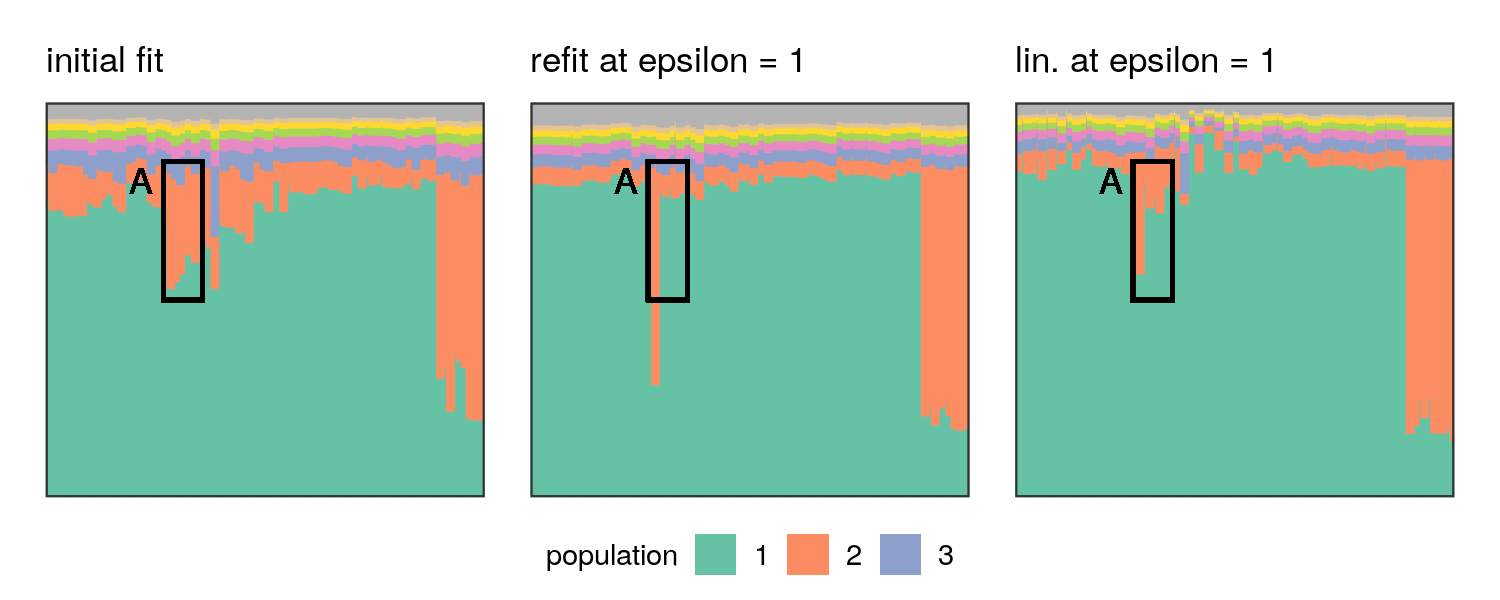
\includegraphics[width = \textwidth]{./figures/bad_admix_example.png}
    \caption*{Inferred admixtures after the worst-case perturbation
     to individuals A.
     Individual $n = 26$ had a large increase in admixture proportion of
     population 2 after the refit. }
  \end{figure}

\end{frame}

\begin{frame}{Limitations of local sensitivity}

  \begin{figure}[!h]
    \centering
    \only<1>{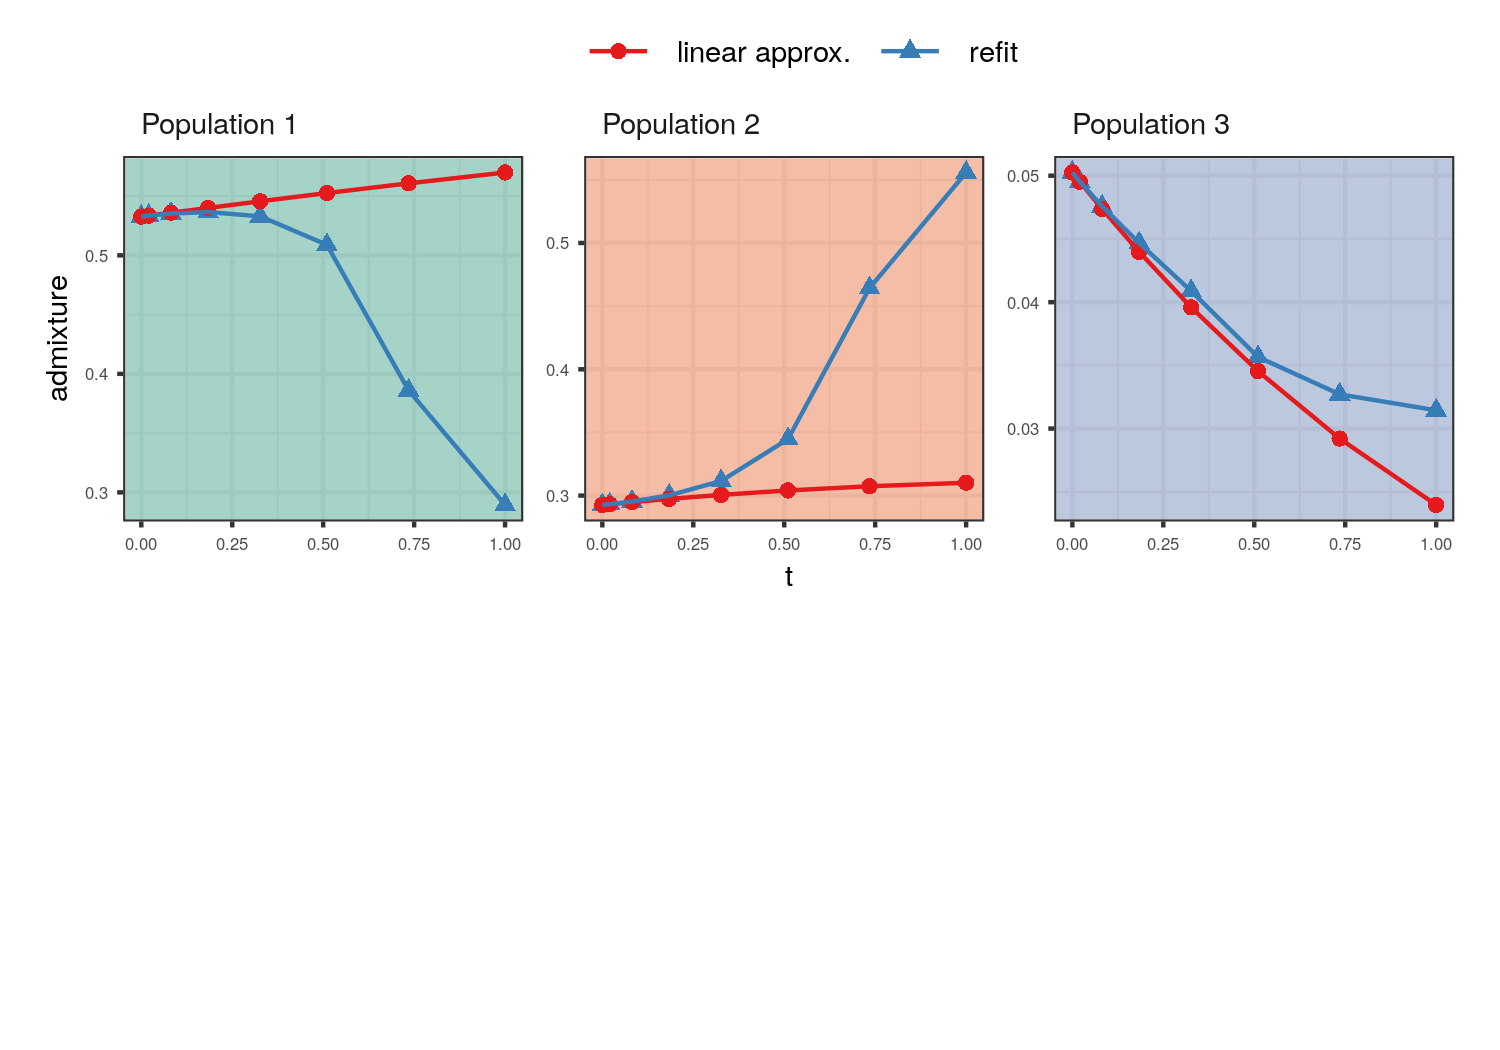
\includegraphics[width = \textwidth]{./figures/bad_admix_example_trace0.png}}%
    \only<2>{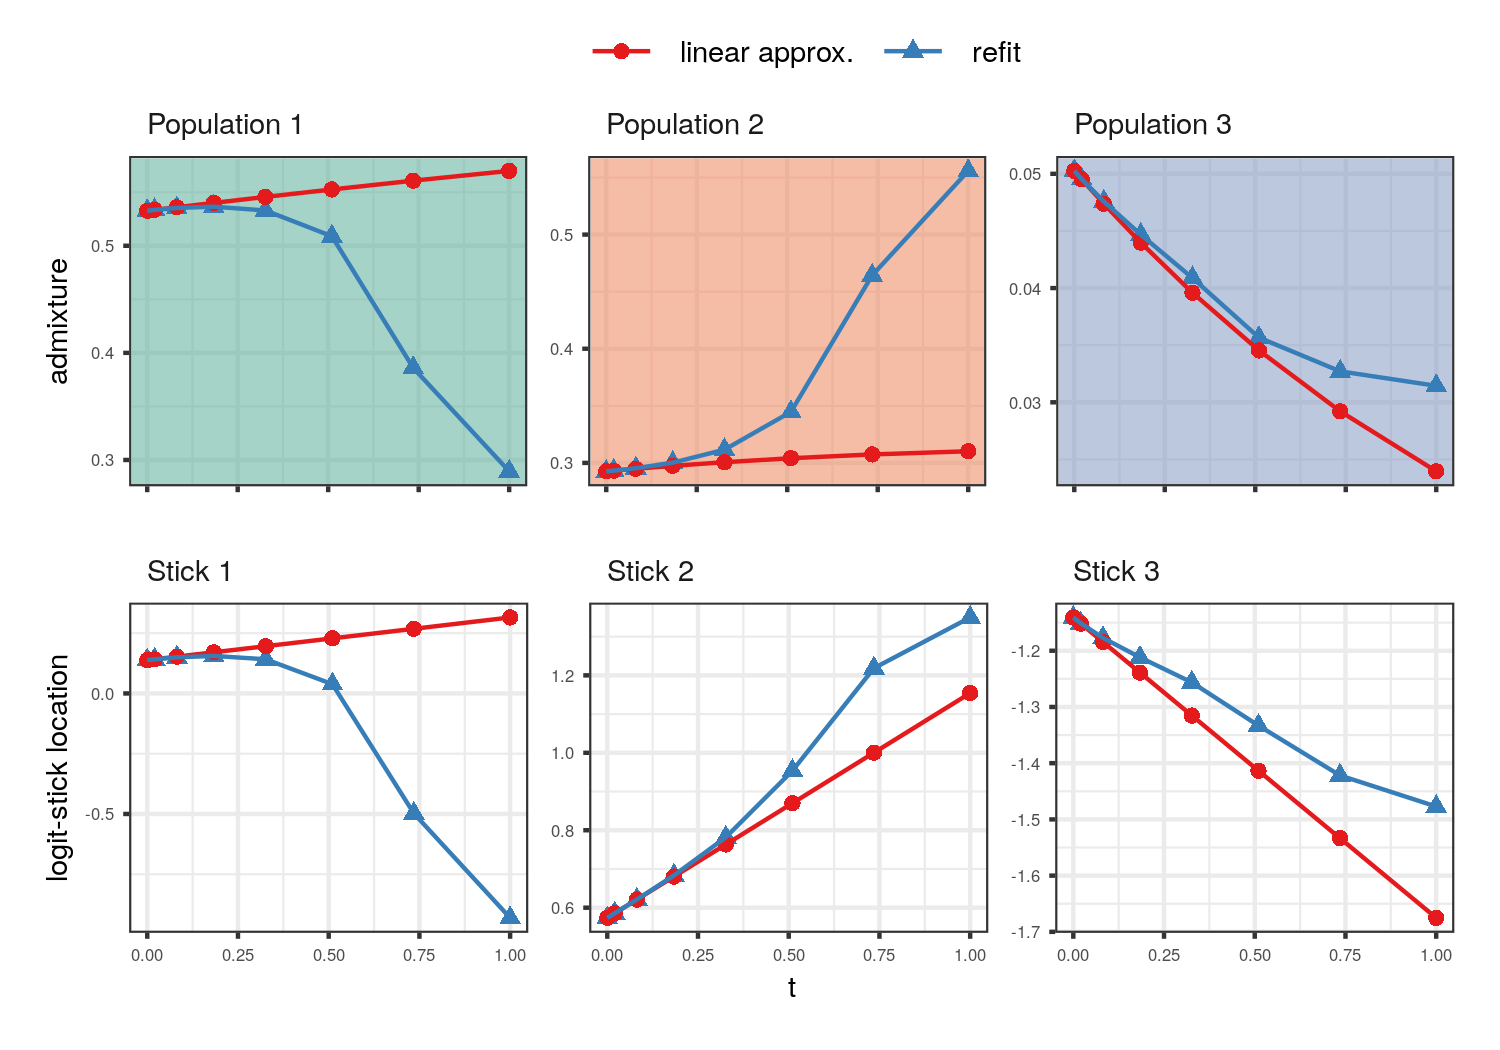
\includegraphics[width = \textwidth]{./figures/bad_admix_example_trace1.png}}%
  \end{figure}

\end{frame}


\begin{frame}{Conclusions}

\begin{itemize}
\item We provide a tool to efficiently evaluate the sensitivity of the variational posterior to prior chioces.
\item Linearizing the variational parameters provides a reasonable alternative
re-optimizing the variational approximation
after model perturbations.
\item The influence function can provide guidance to find particularly sensitive model perturbations.
\end{itemize}

\end{frame}


\begin{frame}{References}

{\bf A workshop paper: }\newline
Runjing Liu, Ryan Giordano, Michael I. Jordan, Tamara Broderick. \newline
“Evaluating Sensitivity to the Stick Breaking Prior in Bayesian Nonparametrics.”
\newline {\color{blue}\url{https://arxiv.org/pdf/1810.06587.pdf}}

\vspace{1em}

{\bf Code: }\newline
Paragami: parameter folding and flattening for optimization problems \newline
{\color{blue}\url{https://github.com/rgiordan/paragami}}

Vittles: library for sensitivity analysis in optimization problems \newline
{\color{blue}\url{https://pypi.org/project/vittles/}}

JAX: composable transformations of Python+NumPy programs \newline
{\color{blue}\url{https://github.com/google/jax}}


\end{frame}


\end{document}
